%----------------------------------------------------------------------------
%----------------------------------------------------------------------------
%				    	SETUP
%----------------------------------------------------------------------------
%----------------------------------------------------------------------------

\documentclass[12pt]{article}

%----------------------------------------------------------------------------
%			  	   PACKAGES
%----------------------------------------------------------------------------

%% Fonts and Symbols
%% --------------------------
\usepackage[T1]{fontenc}			% better font encoding
\usepackage[utf8]{inputenc}		% better font encoding
%\usepackage[usenames,dvipsnames,svgnames,table]{xcolor}		% allow colour
\usepackage{amsmath,amssymb,amsthm,textcomp, xfrac}		% math symbols, etc
%\usepackage{color}
\usepackage[hidelinks]{hyperref}	% hyperlinks, see config in LAYOUT AND STYLING


%% Graphics
%% --------------------------
\usepackage{graphicx}			% allow insertion of images
\graphicspath{ {./graphics/} }		% the relative path to the graphics folder
\usepackage{subfigure}			% allows subfigures (a), (b), etc
%\usepackage{tikz}				% vector graphics
%\usepackage{pgfplots}			% plots in vector graphics


%% Tables
%% --------------------------
\usepackage{booktabs}			% better tables, discourages vertical rulings
%\usepackage{tabularx}
%\usepackage{enumerate}		
\usepackage{multicol}			%allow multi columns


%% Layout Alteration
%% --------------------------
\usepackage{lastpage}
\usepackage{fancyhdr}			% see config in LAYOUT AND STYLING
\usepackage{fullpage}			% set full page margins
%sideways figures
\usepackage{rotating}
%\usepackage{pdflscape}
\usepackage{parskip}			% disable indents
\usepackage{subfigure}			% allows for subfigures to have their own label
\usepackage{caption}			% line breaks in captions with \\

%% Units
%% --------------------------
\usepackage{siunitx}			% has S (decimal align) column type
\sisetup{input-symbols = {()},  % do not treat "(" and ")" in any special way
         group-digits  = false} % no grouping of digits
%\sisetup{load-configurations = abbreviations}
%\sisetup{per-mode = symbol}
%\usepackage{cancel}


%% Misc
%% --------------------------
%\usepackage{mhchem}			% chemistry


%----------------------------------------------------------------------------
%		     MACROS AND COMMANDS
%----------------------------------------------------------------------------

%type Y - even column width - centered
% must include tabularx package
%\newcolumntype{Y}{>{\centering\arraybackslash}X}	

% Defines a new command for the horizontal lines, change thickness here
\newcommand{\HRule}{\rule{\linewidth}{0.5mm}} 	

% ???
\newcommand{\linia}{\rule{\linewidth}{0.5pt}}

% scientific notation  use \e
\providecommand{\e}[1]{\ensuremath{\times 10^{#1}}}

% override S column type with centered text column
\newcommand{\textcol}[1]{\multicolumn{1}{c}{#1}}

% I'm sick of writing rms in subscript
\newcommand{\rms}{\ensuremath{_{rms}}}

%----------------------------------------------------------------------------
%		   	LAYOUT AND STYLING
%----------------------------------------------------------------------------

% custom footers and headers
% must include fancyhdr package
\pagestyle{fancy}
\lhead{}
\chead{}
\rhead{}
\lfoot{}
\cfoot{\thepage\ of \pageref{LastPage}}
\rfoot{}
\renewcommand{\headrulewidth}{0pt}
\renewcommand{\footrulewidth}{0pt}


%%section style
%\usepackage{titlesec}
%\titleformat{\section}[runin]
%{\normalfont\bfseries}
%{\thesection.}{.5em}{}[]
%
%\titleformat{\subsection}[runin]
%{\normalfont\bfseries}
%{\thesubsection}{.5em}{}[]
%\setcounter{secnumdepth}{0} %dont number sections

%\hypersetup{
%%    	colorlinks=false, 		% set true if you want colored links
%   		linktoc=all,     			% set to all if you want both sections and subsections linked
%%  		linkcolor=blue,  			% choose some color if you want links to stand out
%}


%----------------------------------------------------------------------------
%----------------------------------------------------------------------------
%				   DOCUMENT
%----------------------------------------------------------------------------
%----------------------------------------------------------------------------

\begin{document}

%----------------------------------------------------------------------------
%				    TITLE PAGE
%----------------------------------------------------------------------------

\begin{titlepage}

\center
 
% Header
\textsc{\LARGE University of Victoria}\\[1cm] 	% Name of your university/college
\textsc{\Large ELEC 250}\\[0.5cm] 			% Major heading such as course name
\textsc{\large Linear Circuits I}\\[0.5cm] 		% Minor heading such as course title


% Lab Title
\HRule \\[0.4cm]
{ \huge \bfseries Lab 4 - Resonance and Power}\\[0.2cm] % Title of your document
\HRule \\[1.5cm]
 
 
%Lab Instructor Details
\begin{minipage}{0.7\textwidth}
\begin{flushleft} 

\large\emph{Instructor:} \\
Dr. Nikitas \textsc{Dimopoulos} \\
\vspace{12 pt}
\emph{Teaching Assistant:} \\
Zhen \textsc{Liu}

\end{flushleft}
\end{minipage}
~
%% No content here, but it keeps the alignment of the instructor/TA
%% box correct.
%% Consider revising.
\begin{minipage}{0.1\textwidth}
\begin{flushright} \large
%Dr. Barbara \textsc{Sawicka} \\
\vspace{12 pt}
%\emph{Teaching Assistant:} \\
%Vahid \textsc{Moradi}
\end{flushright}
\end{minipage}\\[2cm]


% Lab members
\Large Clayton \textsc{Kihn}
\large V00794569	\\
\Large Yves \textsc{Senechal}
\large V00213837	\\
\Large Tyler \textsc{Stephen}
\large V00812021	\\
A01 - B01\\[1.5cm] 


% Date
{\large \today}\\ % Date, change the \today to a set date if you want to be precise

% Logo
\begin{figure}[b]	 % put logo at bottom of the page
	\centering
	\includegraphics[scale=0.3]{UVic_logo}
\end{figure}

\end{titlepage}

%----------------------------------------------------------------------------
%			  TABLE OF CONTENTS
%----------------------------------------------------------------------------

%\tableofcontents
%\pagebreak

%\listoffigures
%\pagebreak

%----------------------------------------------------------------------------
%				    BODY
%----------------------------------------------------------------------------

\section{Object}\label{sec:object}
This lab will study series resonance as well as the measurement of power in a circuit using a wattmeter.

\section{Series Resonance}\label{sec:resonance}
\subsection{Procedure}\label{sec:res_procedure}
\begin{figure}[h]
	\centering
	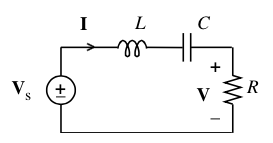
\includegraphics[scale=0.75]{resonance_diagram}
	\caption{Circuit diagram of resonant RLC circuit \\ $L$ = 1.00 mH, $C$ = 22 nF, $R$ = 43.50 $\Omega$}
	\label{fig:res_diagram}
\end{figure}

\subsection{Results}\label{sec:res_results}
Table \ref{table:resonance} is located at the end of this report.

\begin{figure}[h]
	\centering
	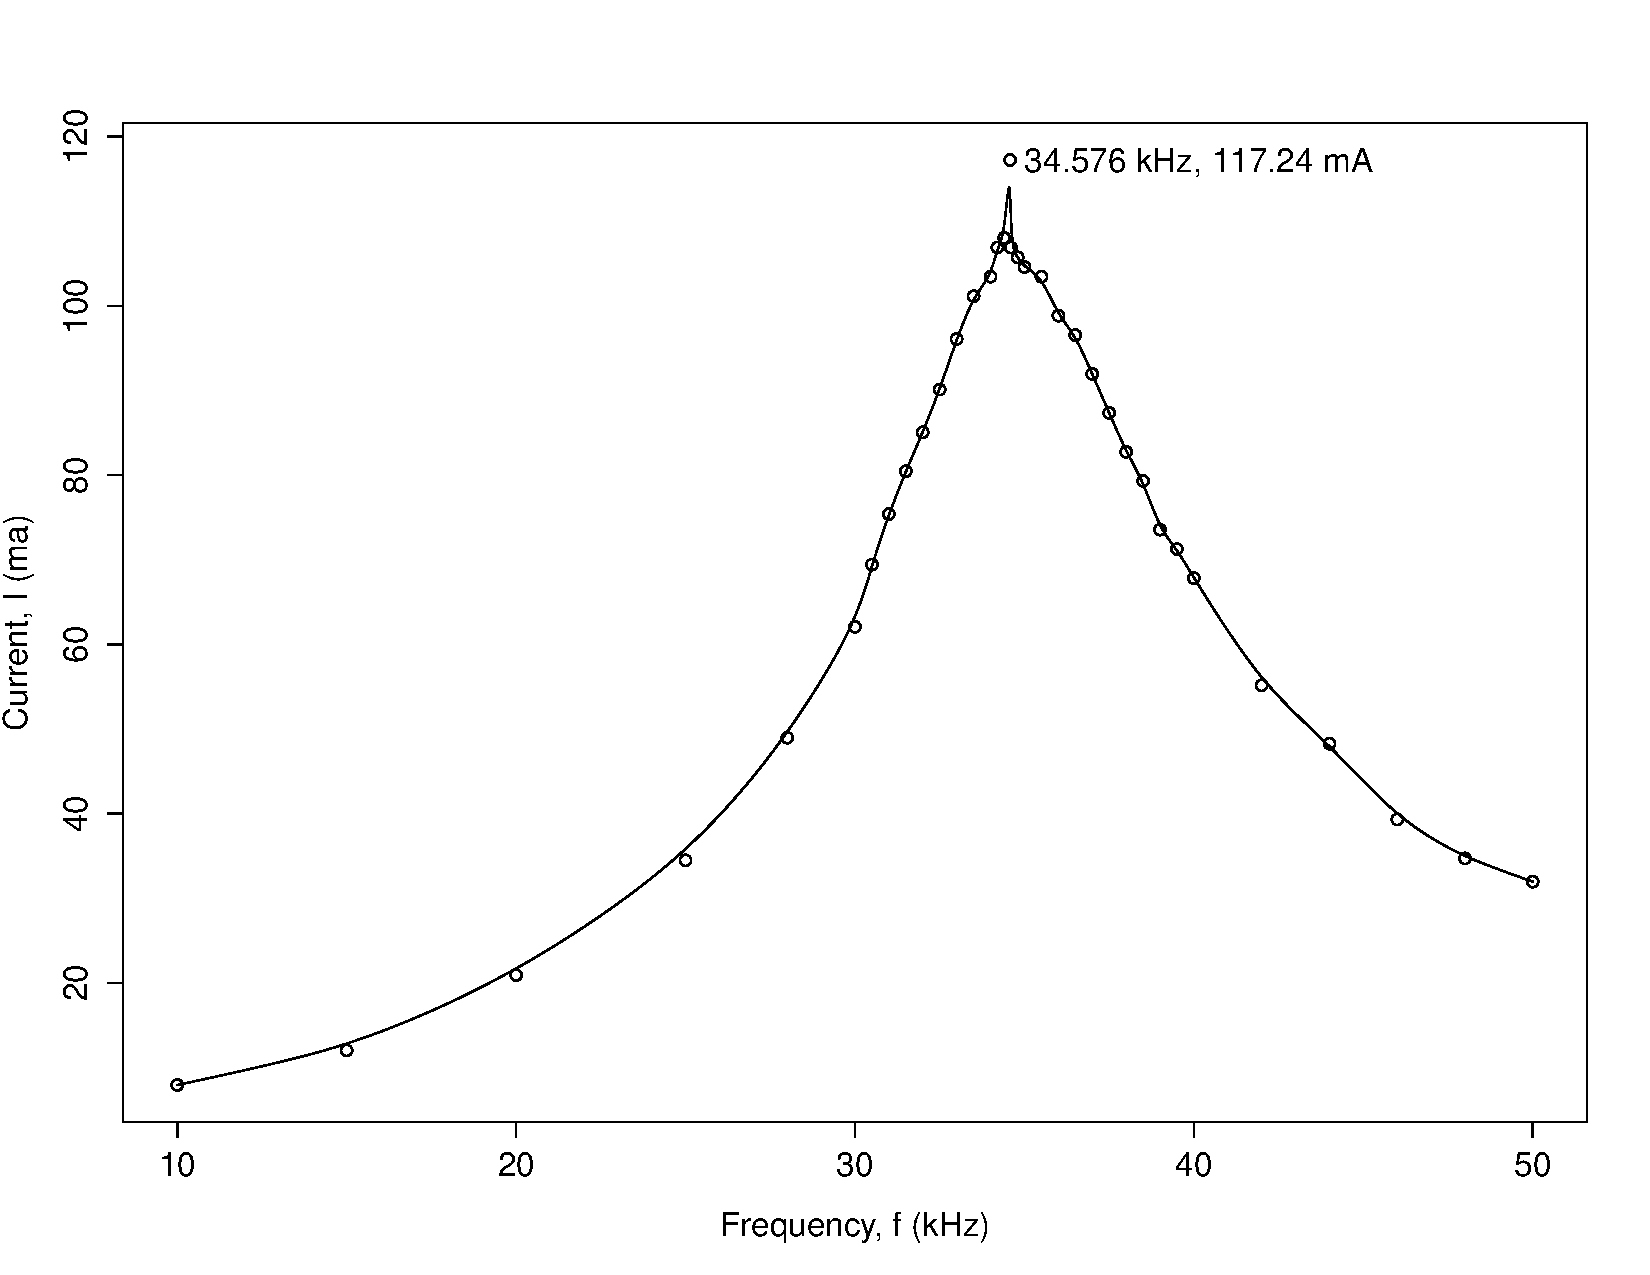
\includegraphics[scale=0.5]{resonance_plot}
	\caption{Current through RLC circuit as frequency passes through resonance}
	\label{figure:res_graph}
\end{figure}

find $f_0$, $f_1$, $f_2$, $B$ by interpolating the graph. (hint, using the data table will be the best way to find $f_1$ and $f_2$ since we know they occur at $\theta = \pm45^{\circ}$)

\subsection{Discussion}\label{sec:res_discussion}
How do $f_0$, $f_1$, $f_2$, $B$ compare with expected values?

\section{Power Measurement}\label{sec:power}
\subsection{Procedure}\label{sec:pow_procedure}
The power factor $pf$ is the ratio of true versus apparent power. A leading $pf$ is achieved in an $RC$ circuit, while a lagging $pf$ is the result of a $RL$ circuit. Two experiments were performed where a leading and lagging $pf$ were obtained separately. The block diagram in Figure \ref {fig:comp_diagram} represents the physical setup of the experiment: $(a)$ a high-wattage component board that carries a 200$\Omega$ resistor, a 300$m$H inductor, and a 10$\mu$F capacitor, $(b)$ a variac with an isolation transformer used to reduce the voltage to 50V$_{rms}$, and $(c)$ (not shown) a wattmeter between the isolation transformer and the component board to measure real power. The diagram in Figure \ref {fig:pf_circuit} represents the electrical $RC$ circuit; the $RL$ circuit is similar with the substitution of and inductor $L$ in place of the capacitor $C$.

\begin{figure}[h]
	\centering
	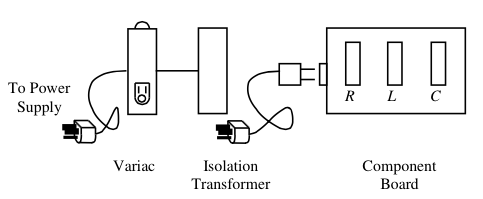
\includegraphics[scale=0.75]{power_components}
	\caption{Block diagram of circuit components\\$R$ = 200 $\Omega$, $L$ = 300 $m$H, $C$ = 10 $\mu$F}
	\label{fig:comp_diagram}
\end{figure}

\begin{figure}[h]
	\centering
	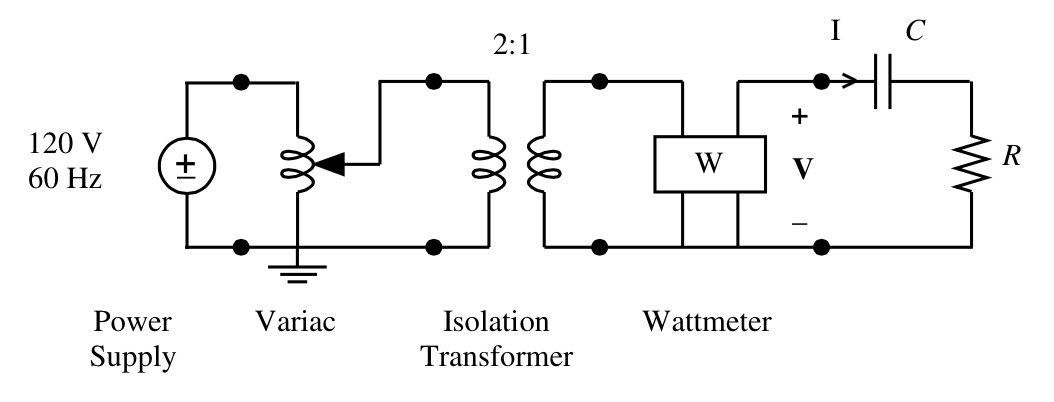
\includegraphics[scale=0.75]{pf_circuit}
	\caption{$RC$ $pf$ measurement circuit setup}
	\label{fig:pf_circuit}
\end{figure}

\subsection{Results}\label{sec:pow_results}

The first part, a $RC$ circuit was constructed to measure its power consumption. With a 200$\Omega$ resistor, a 10$\mu$F capacitor, and the voltage set to 49.94V$_{rms}$, the wattmeter measured a current of 151.0$m$A with power consumption of 4.55W. A digital multimeter (DMM) placed across the resistor indicated V$_R$ = 30.06V$_{rms}$. Using the equation

\begin{equation}
	P = \frac{V_{R}^2}{R} 
	\label{eqn:P}
\end{equation}

the true power $P$ is calculated to be 4.52W. Similarly, the apparent power $S$ is calculated using the equation,

\begin{equation}
	S = {V_{rms}}{I_{rms}}
	\label{eqn:S} 
\end{equation}

and results to $S$ = 7.54VA. The $pf$ can be estimated using 

\begin{equation}
	pf = \frac{P}{S}
	\label{eqn:pf}
\end{equation}

which yeilds a power factor of 0.6034. The $pf$ was then be measured to be 0.6019 by the following relationship.

\begin{equation}
	pf = \frac{P}{V\rms I\rms}
	\label{eqn:pf_rms}
\end{equation}

The relationship of the reactive power $Q$, true power $P$, and apparent power $S$ is represented by the following equation, which results in $Q$ = 6.014VAR.

\begin{equation}
	Q = \sqrt{S^2 - P^2}
	\label{eqn:Q}
\end{equation}

An $RL$ circuit was constructed for the second part with a 200$\Omega$ resistor, a 300 $m$H inductor, and the voltage set to 50.09V$_{rms}$. The wattmeter in turn measured a current of 181.5$m$A with power consumption of 7.16W. A digital multimeter (DMM) placed across the resistor indicated V$_R$ = 36.10V$_{rms}$. 

Using equation \ref{eqn:P}, the true power $P$ is expected to be 6.52W. With the relationship of equation \ref{eqn:S}, the apparent power results in $S$ = 9.09VA.

A $pf$ of 0.7876 is estimated using equation \ref{eqn:pf}; however, the $pf$ was measured to be 0.7207 using the relationship of equation \ref{eqn:pf_rms}.

Using equation \ref{eqn:Q}, the reactive power $Q$ results in a value of 5.602VAR.


\begin{table}[h]
	\centering
	\begin{tabular}{S S S S S S S S S}
	\toprule
	& & & & & \multicolumn{2}{c}{$P$ (W)} & \multicolumn{2}{c}{$pf$} \\
		\textcol{Circuit}& 
		\textcol{$V\rms$ (V)} & 
		\textcol{$I\rms$ (mA)} & 
		\textcol{$V_R$ (V)} & 
		\textcol{$Q$ (VAR)} &
		\textcol{$measured$} & 
		\textcol{$\frac{V_R ^2}{R}$} &  
		\textcol{$\frac{P}{S}$} & 
		\textcol{$\frac{V_R}{Vrms}$} \\ 
	\midrule
		RC	& 49.94	& 151.0	& 30.06	& 6.014	& 4.55	& 4.54	& 0.6034	& 0.6019	\\
		RL	& 50.09	& 181.5	& 36.10 & 5.602	& 7.16	& 6.55	& 0.7876	& 0.7207 	\\ 
	\bottomrule
	\end{tabular}
	\caption{Power measurements in RC and RL circuits}
	\label{table:power}
\end{table}

\subsection{Discussion}\label{sec:pow_discussion}
The $RC$ circuit yielded similar power measurement results to those expected. In this circuit the difference between measured and calculated real power $P$ and power factor $pf$ was 0.664\% and 0.249\% respectively, which is negligible and expected when using non-ideal components.

The $RL$ circuit, however, showed slightly bigger discrepancies. The difference between measured and calculated $P$ and $pf$ was 8.94\% and 8.49\% respectively. From past experiments, these results can be expected due to the nature of inductors. Heat will increase the internal resistance, which ultimately skews the results.


\section{Conclusion}\label{sec:conclusion}

\newpage
% lol, I am a scrub and can't fit the title + table on the same page.
%\section*{Appendix}\label{app}
%\subsection{Data for resonance in RLC circuit}

\begin{table}[h]
\centering
\begin{tabular}{@{}SSSS@{}}
\toprule
\textcol{Frequency} & 
	\textcol{Resistor Voltage} & 
	\textcol{Current} & 
	\textcol{Phase Shift} \\ 
\textcol{$f$ (kHz)} &
	\textcol{$V_r$ (V)} &
	\textcol{$I$ (mA)} &
	\textcol{$\theta$ ($^{\circ}$)} \\
\midrule
10.000 & 0.345 & 7.931   & -85.0 \\
15.000 & 0.523 & 12.023  & -82.0 \\
20.000 & 0.910 & 20.920  & -76.0 \\
25.000 & 1.500 & 34.483  & -69.0 \\
28.000 & 2.130 & 48.966  & -61.0 \\
30.000 & 2.700 & 62.069  & -51.5 \\
30.500 & 3.020 & 69.425  & -47.0 \\
31.000 & 3.280 & 75.402  & -43.5 \\
31.500 & 3.500 & 80.460  & -38.0 \\
32.000 & 3.700 & 85.057  & -34.5 \\
32.500 & 3.920 & 90.115  & -28.0 \\
33.000 & 4.180 & 96.092  & -22.0 \\
33.500 & 4.400 & 101.149 & -15.0 \\
34.000 & 4.500 & 103.448 & -8.0  \\
34.200 & 4.650 & 106.897 & -5.0  \\
34.400 & 4.700 & 108.046 & -2.3  \\
34.576 & 5.100 & 117.241 & -0.1  \\
34.600 & 4.650 & 106.897 & 0.8   \\
34.800 & 4.600 & 105.747 & 3.8   \\
35.000 & 4.550 & 104.598 & 6.8   \\
35.500 & 4.500 & 103.448 & 13.5  \\
36.000 & 4.300 & 98.851  & 20.0  \\
36.500 & 4.200 & 96.552  & 25.8  \\
37.000 & 4.000 & 91.954  & 31.5  \\
37.500 & 3.800 & 87.356  & 35.7  \\
38.000 & 3.600 & 82.759  & 40.0  \\
38.500 & 3.450 & 79.310  & 43.5  \\
39.000 & 3.200 & 73.563  & 47.2  \\
39.500 & 3.100 & 71.264  & 50.0  \\
40.000 & 2.950 & 67.816  & 53.0  \\
42.000 & 2.400 & 55.172  & 61.0  \\
44.000 & 2.100 & 48.276  & 66.0  \\
46.000 & 1.710 & 39.310  & 69.5  \\
48.000 & 1.510 & 34.713  & 72.0  \\
50.000 & 1.390 & 31.954  & 74.7  \\ 
\bottomrule
\end{tabular}
\caption{Change in current through resistor in RLC circuit as source frequency passes through resonance}
\label{table:resonance}
\end{table}

%----------------------------------------------------------------------------
%				  LaTeX TIPS
%----------------------------------------------------------------------------
%
%\pagebreak
%
%\section{LaTeX Tips}\label{sec:tips}
%Check the source file for additional information in the comments.
%\subsection{Symbols}\label{sec:symbols}
%Most math symbols and all equations are bounded by \$ delimiters. \verb|$ A=\pi r^{2} $| produces $ A=\pi r^{2} $. To find the appropriate symbol you will have to use a LaTeX IDE with a built in symbol editor or use another program to produce the code and copy-and-paste it into your document.
%
%\subsection{Figures}\label{sec:figures}
%\begin{verbatim}
%\begin{figure}[h]
%	\centering
%	\includegraphics[width=0.75\textwidth]{Uvic_logo}
%	\caption{A logo used by the University of Victoria}
%	\label{fig:uvic_logo}
%\end{figure}
%\end{verbatim}
%
%\begin{figure}[h] 	% placement in document [htbp]: here, top, bottom, special page
%	\centering		% centers the image
%	\includegraphics[width=0.75\textwidth]{Uvic_logo} 	
%		% will search root directory and anything listed
%		% in \graphicspath for the image
%		% it is common to specify [width=0.5\textwidth] as an agument
%		% \textwidth can be used as a variable for the entire pagewidth.
%		% 0.5\textwidth refers to 50% of the page.
%	\caption{A logo used by the University of Victoria}
%	\label{fig:uvic_logo}
%\end{figure}
%
%A good tutorial for the use of figures can be found at: \url{http://en.wikibooks.org/wiki/LaTeX/Floats,_Figures_and_Captions}
%
%\pagebreak
%\subsection{Tables}\label{sec:tables}
%\begin{verbatim}
%\begin{table}[h]
%	\centering
%	\begin{tabular}{llr}
%		\hline
%		\multicolumn{2}{c}{Item} \\
%		\cline{1-2}
%			Animal   	& Description 	& Price (\$) \\
%		\hline
%			Gnat		& per gram	& 13.65      \\
%				        & each       	& 0.01       \\
%			Gnu		& stuffed     	& 92.50      \\
%			Emu		& stuffed		& 33.33      \\
%			Armadillo	& frozen		& 8.99       \\
%		\hline
%	\end{tabular}
%	\caption{Exotic meat prices}
%	\label{table:meats}
%\end{table}
%\end{verbatim}
%
%\begin{table}[h]			% placement in document [htbp]: [h]ere, [t]op, [b]ottom, special [p]age
%	\centering
%	\begin{tabular}{llr}	% specifies the number of columns and their justification
%					% columns can be [l]eft-justified, [c]entered, [r]ight-justified
%					% the number of arguments after {tabular} corresponds to the number of columns
%					% vertical lines can be added by placing | vertical bars in the argument
%					% e.g. { | c c c | } has three centered columns with vertical lines at the ends
%					% of the table
%					% { | c | c | c | } has vertical lines separating all cells
%
%		\hline		% a horizontal line
%		
%		\multicolumn{2}{c}{Item} \\		% {number of columns to span}{lcr}{title}
%								% \\ indicates the end of a line
%								
%		\cline{1-2}		% \cline[ i - j } : line that spans columns i to j
%		
%			Animal   	& Description 	& Price (\$) \\	% & separates data between cells
%											% && indicates a blank cell
%											% \\ must end every row
%		\hline
%			Gnat		& per gram	& 13.65      \\
%				        & each       	& 0.01       \\
%			Gnu		& stuffed     	& 92.50      \\
%			Emu		& stuffed		& 33.33      \\
%			Armadillo	& frozen		& 8.99       \\
%		\hline
%	\end{tabular}
%	\caption{Exotic meat prices}
%	\label{table:meats}
%\end{table}
%\textit{Apparently} tables are more readable if the vertical rulings are omitted. I'm inclined to agree.\\
%A good tutorial for the use of tables can be found at: \url{http://en.wikibooks.org/wiki/LaTeX/Tables}
%
%\subsection{Labels and References}\label{sec:labels_and_refs}
%LaTeX's dynamic referencing system gives it an advantage over other multi-user document tools. References point to assigned labels rather than a pre-defined numbering. Changing the order and number of references will leave the citations untouched if label referencing is used.
%
%
%The \verb|\label{}| tag should be attached to all sections, figures and tables. To reference these elements, use the \verb|\ref{}| command. To reference the table in Section \ref{sec:tables}, you would write \verb|Table \ref{table:meats}| which will appear as Table \ref{table:meats}.
%
%
%A consistent naming schema will make collaboration easier. Labels should be implemented with the corresponding prefix:
%\begin{table}[h]
%	\centering
%	\begin{tabular}{ l l }
%	Sections		& \verb|{sec:}|		\\
%	Figures		& \verb|{fig:}|		\\
%	Tables		& \verb|{table:}|		\\
%	\end{tabular}
%\end{table}
%
%You may encounter a situation where a citation or page number appears as \verb|??|. This often occurs when major changes have occured to the reference or page order. The LaTeX compiler requires two executions of the typesetting function to correctly address the references: one to build the .aux file and another to read from it. The compiler is often nice enouch to pass a warning when the .aux file has undergone significant changes to its references and prompts you do another typesetting.
%
%\subsection{Resources}\label{sec:resources}
%\begin{itemize}
%	\item \underline{\href{https://www.youtube.com/user/14mech14/videos}{Video playlist} } from McMaster that covers the installation and use of LaTeX. Uses TeXShop for examples. Covers document setup, tables, figures, bibliographies and some other stuff I haven't watched yet.
%\end{itemize}

%----------------------------------------------------------------------------
%----------------------------------------------------------------------------
%			DO NOT DELETE BELOW
%----------------------------------------------------------------------------
%----------------------------------------------------------------------------

\end{document}